\documentclass[12pt,a4paper]{extarticle}
\usepackage[left=25mm,right=20mm,top=20mm,bottom=20mm]{geometry}
\usepackage{fontspec}
\IfFontExistsTF{Times New Roman}{\setmainfont{Times New Roman}}{\setmainfont{Liberation Serif}}
\setmonofont{DejaVu Sans Mono}[Scale=0.8]
\usepackage{polyglossia}
\setdefaultlanguage{russian}
\setotherlanguage{english}
\usepackage{amsmath,amssymb,graphicx,booktabs,tabularx,array}
\usepackage{setspace,caption,float,enumitem,titlesec}
\usepackage[unicode,hidelinks]{hyperref}
\hypersetup{pdfauthor={Шешуков Евгений Игоревич},pdflang={ru-RU}}
\setstretch{1.15}
\setlength{\parindent}{1.25cm}
\setlength{\parskip}{3pt}
\setlength{\emergencystretch}{2em}
\setlength{\tabcolsep}{5pt}
\setlength{\intextsep}{8pt}
\renewcommand{\arraystretch}{1.18}
\captionsetup{font=small,labelsep=colon,justification=centering}
\setlist{nosep,topsep=5pt,leftmargin=1.4cm}
\titleformat{\section}{\large\bfseries}{\thesection.}{0.5em}{}
\titleformat{\subsection}{\normalsize\bfseries}{\thesubsection.}{0.5em}{}
\titlespacing*{\section}{0pt}{12pt}{7pt}
\titlespacing*{\subsection}{0pt}{9pt}{4pt}
\setlength{\abovedisplayskip}{7pt}
\setlength{\belowdisplayskip}{7pt}
\widowpenalty=10000
\clubpenalty=10000
\raggedbottom
\newcommand{\code}[1]{\texttt{\small #1}}
\newcommand{\reporttitle}[2]{%
\hypersetup{pdftitle={Лабораторная работа №#1. #2}}
\begin{titlepage}
\begin{center}
{\bfseries БЕЛОРУССКИЙ ГОСУДАРСТВЕННЫЙ УНИВЕРСИТЕТ\par}
\vspace{4mm}
{\bfseries ФАКУЛЬТЕТ ПРИКЛАДНОЙ МАТЕМАТИКИ\par И ИНФОРМАТИКИ\par}
\vspace{4mm}
Кафедра компьютерных технологий и систем
\vspace{34mm}

{\Large\bfseries ОТЧЁТ ПО ЛАБОРАТОРНОЙ\par РАБОТЕ №#1\par}
\vspace{7mm}
{\Large\bfseries «#2»\par}
\vspace{7mm}
Дисциплина: Компьютерная графика\par
\vspace{3mm}
Вариант 13
\end{center}
\vspace{24mm}
\hfill\begin{minipage}{0.57\textwidth}
\textbf{Выполнил:}\par
студент 3 курса 2 группы\par
Шешуков Евгений Игоревич\par
\vspace{6mm}
\textbf{Преподаватель:}\par
Каркоцкий Александр Геннадьевич
\end{minipage}
\vfill
\begin{center}Минск, 2026\end{center}
\end{titlepage}
\setcounter{page}{2}}

\begin{document}
\reporttitle{1}{Цветовые модели}

\section{Цель и задание}
Изучить цветовые модели и реализовать приложение, которое показывает один цвет в трёх моделях одновременно. Номер в списке группы --- 13, поэтому используется нечётный вариант: CMYK, RGB и HLS.

В каждой модели цвет задаётся числовыми полями, ползунками и двумерной палитрой. При изменении любой компоненты два других представления пересчитываются автоматически.

\subsection*{Компоненты моделей}
\textbf{RGB} описывает сложение красного, зелёного и синего света. Компоненты $R,G,B$ принимают значения от 0 до 255. Нулевые значения дают чёрный цвет, максимальные --- белый.

\textbf{CMYK} описывает доли голубой, пурпурной, жёлтой и чёрной красок. В интерфейсе $C,M,Y,K$ задаются в процентах. В работе используется учебная модель без профилей принтера: свойства бумаги и конкретных красок не учитываются.

\textbf{HLS} разделяет цвет на тон $H$, светлоту $L$ и насыщенность $S$. Тон задаётся углом $0\ldots360^\circ$, светлота и насыщенность --- процентами. При $S=0$ получается серый; при $L=0$ --- чёрный, при $L=100\%$ --- белый. Порядок координат в программе: $H,L,S$.

\section{Математика преобразований}
\subsection{RGB и CMYK}
Перед вычислениями RGB нормируется: $r=R/255$, $g=G/255$, $b=B/255$. Обозначим $v=\max(r,g,b)$. Тогда
\begin{equation}
 k=1-v,\qquad c=1-\frac{r}{v},\qquad m=1-\frac{g}{v},\qquad y=1-\frac{b}{v}.
\end{equation}
При $v=0$ отдельно возвращается $(c,m,y,k)=(0,0,0,1)$, чтобы избежать деления на ноль. Для отображения значения умножаются на 100.

Обратное преобразование использует нормированные $c,m,y,k$:
\begin{equation}
 R=255(1-c)(1-k),\quad G=255(1-m)(1-k),\quad B=255(1-y)(1-k).
\end{equation}
Например, CMYK $(50,50,50,50)\%$ даёт RGB $(63.75,63.75,63.75)$. Тот же RGB получается при CMYK $(0,0,0,75)\%$. Поэтому программа сохраняет введённые координаты исходной модели, а не заменяет их результатом обратного пересчёта.

\clearpage
\subsection{RGB и HLS}
Для нормированных $r,g,b$ вычисляются
\begin{equation}
 v=\max(r,g,b),\quad n=\min(r,g,b),\quad d=v-n,\quad l=\frac{v+n}{2}.
\end{equation}
Если $d=0$, насыщенность равна нулю, а неопределённый тон условно принимается равным $0^\circ$. Иначе
\begin{equation}
 s=\frac{d}{1-|2l-1|},\qquad
 H=60^\circ\begin{cases}
 ((g-b)/d)\bmod 6,&v=r,\\
 (b-r)/d+2,&v=g,\\
 (r-g)/d+4,&v=b.
 \end{cases}
\end{equation}
В интерфейс возвращаются $H$, $L=100l$ и $S=100s$.

Для перехода из HLS в RGB сначала вычисляются
\begin{equation}
 q=\frac{H\bmod360^\circ}{60^\circ},\quad
 c=(1-|2l-1|)s,\quad x=c(1-|q\bmod2-1|),\quad a=l-\frac{c}{2}.
\end{equation}
По номеру сектора выбирается временная тройка:
\begin{equation}
 (r',g',b')=\begin{cases}
 (c,x,0),&0\le q<1,\\
 (x,c,0),&1\le q<2,\\
 (0,c,x),&2\le q<3,\\
 (0,x,c),&3\le q<4,\\
 (x,0,c),&4\le q<5,\\
 (c,0,x),&5\le q<6.
 \end{cases}
\end{equation}
Окончательно $(R,G,B)=255(r'+a,g'+a,b'+a)$.

\subsection*{Пример расчёта}
Для HLS $(120^\circ,50\%,100\%)$ получаем $q=2$, $c=1$, $x=0$, $a=0$. Следовательно, RGB равен $(0,255,0)$, а CMYK --- $(100,0,100,0)\%$: это чистый зелёный цвет.

Углы $0^\circ$ и $360^\circ$ обозначают один тон. Если пользователь задал тон у чёрного цвета, исходные HLS сохраняются: при последующем увеличении светлоты появляется именно выбранный цвет.

\clearpage
\section{Интерфейс и реализация}
Программа написана на Python с графическим интерфейсом Tkinter. Дополнительные библиотеки не требуются. Формулы находятся в \code{colors.py}, окно и обработчики событий --- в \code{app.py}.

\begin{figure}[H]
\centering
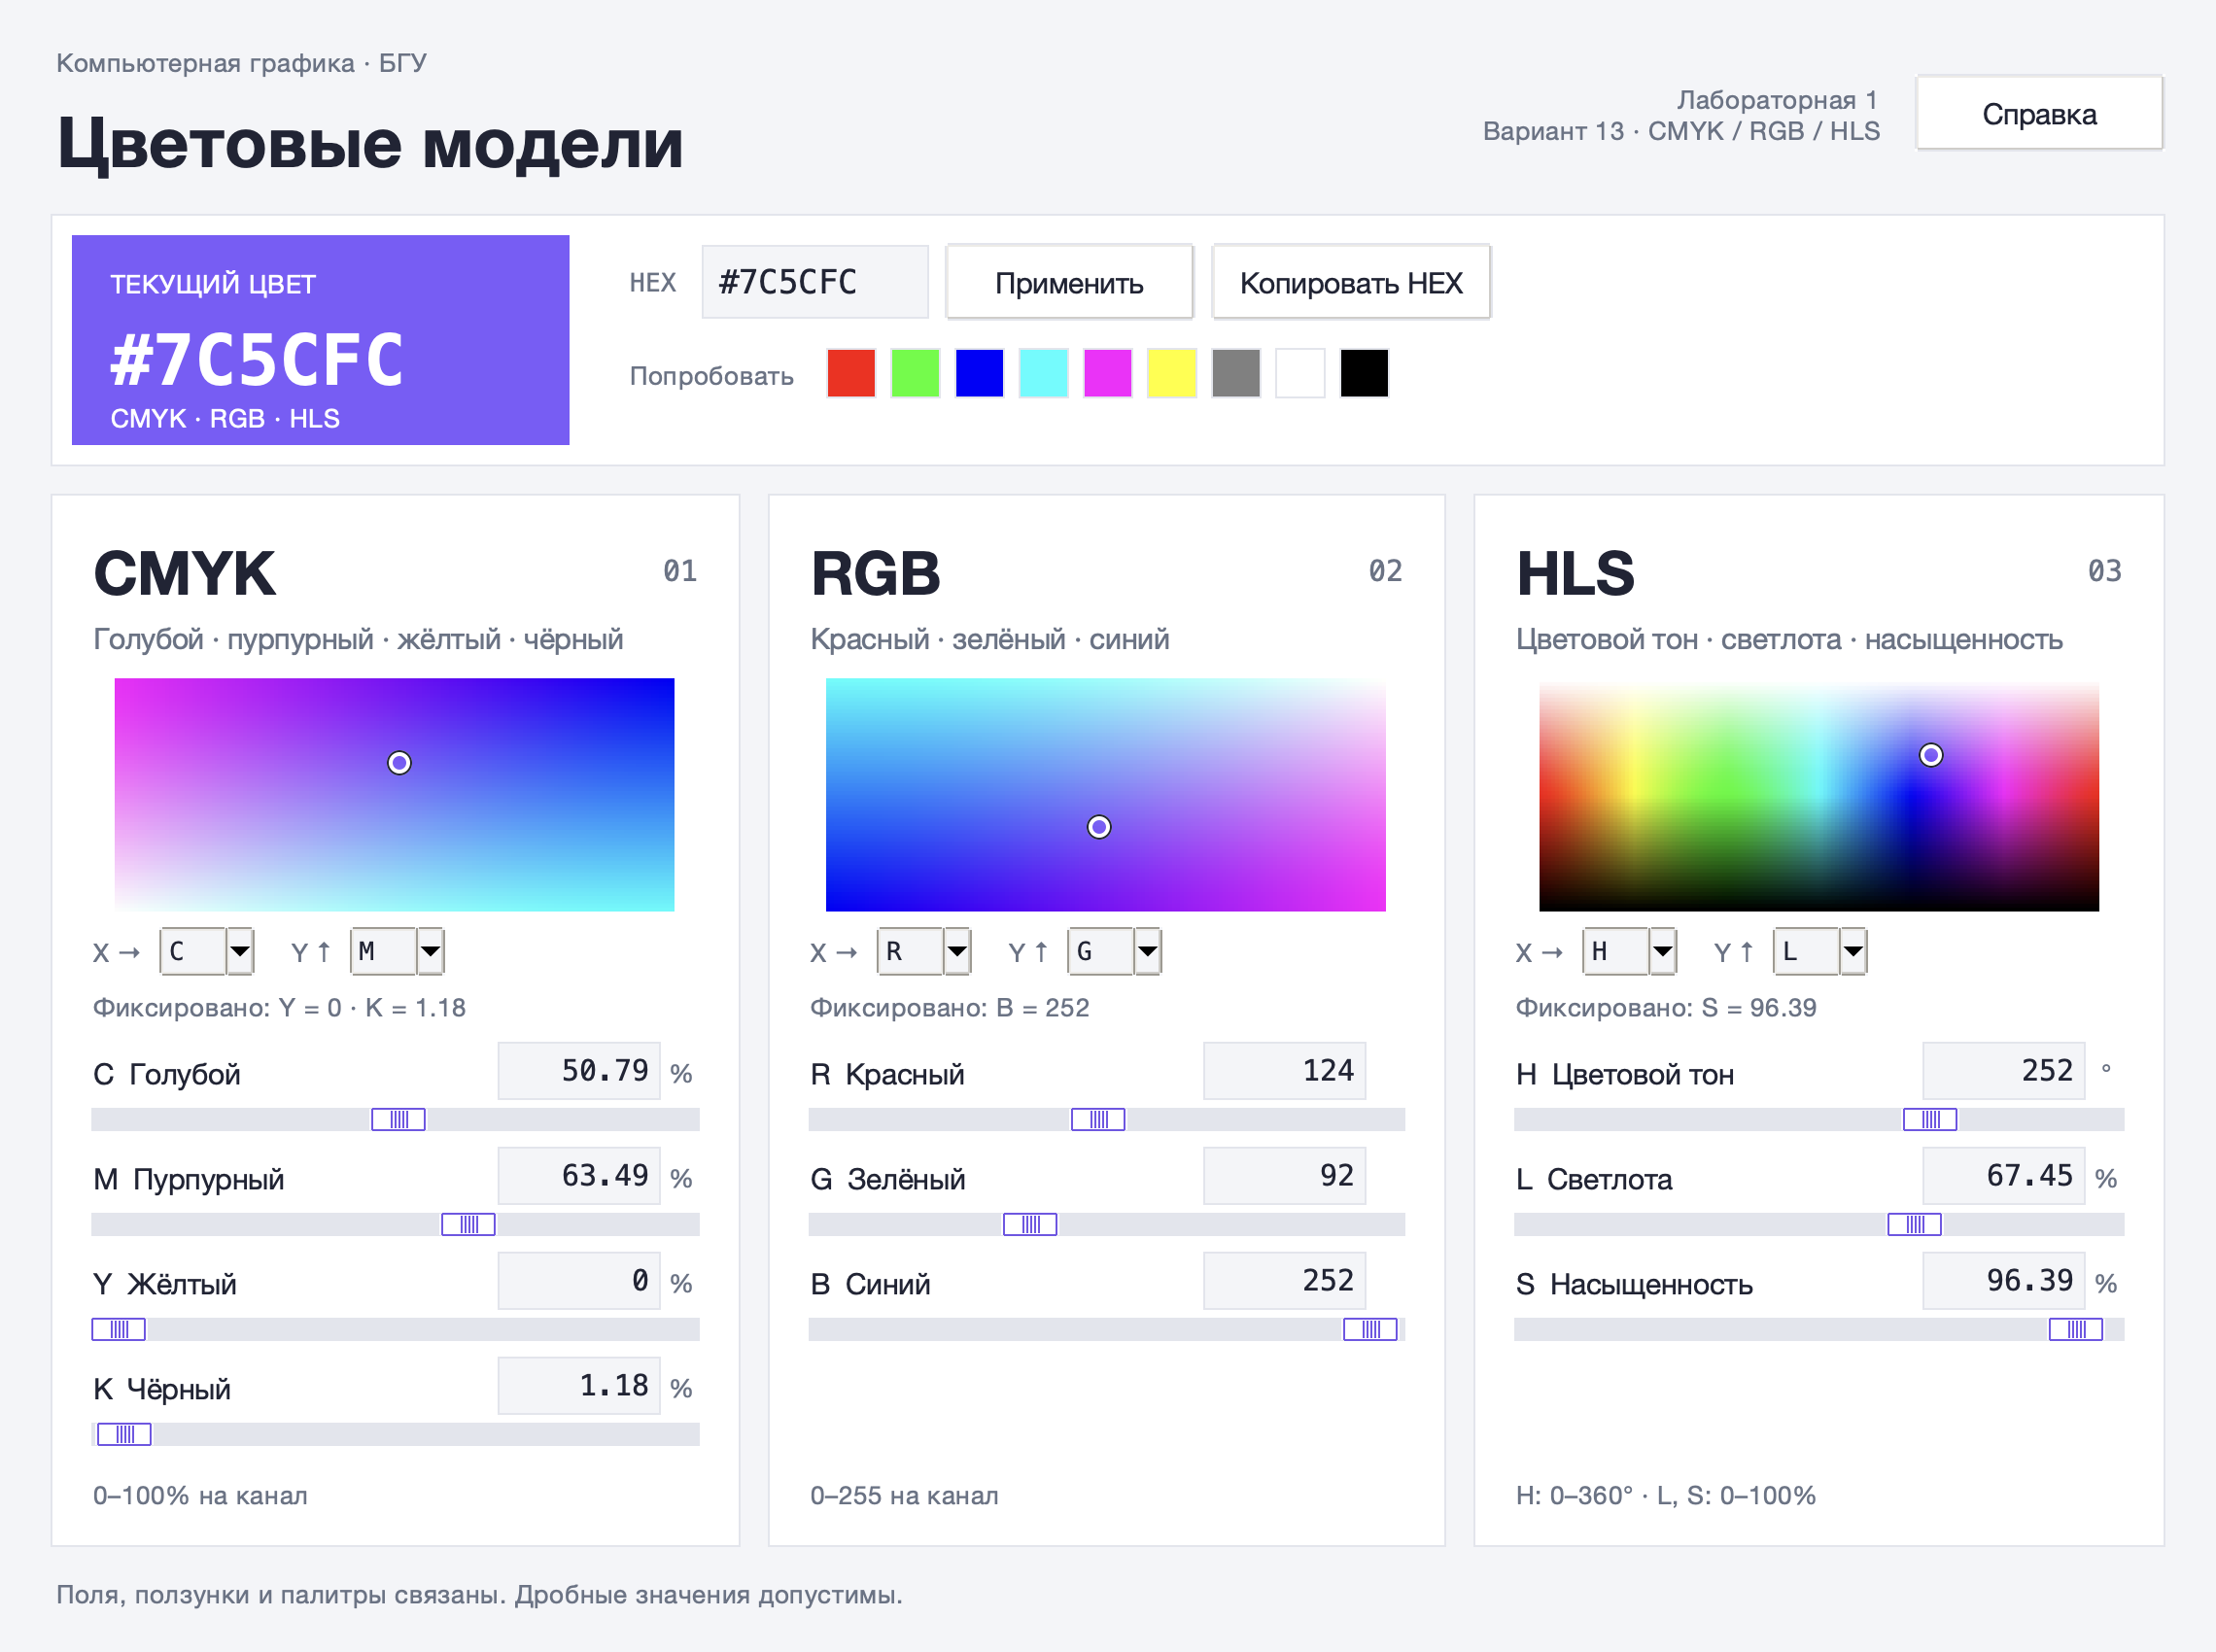
\includegraphics[width=\textwidth]{../docs/screenshot.png}
\caption{Главное окно: один цвет в моделях CMYK, RGB и HLS}
\end{figure}

У каждой модели есть поля, ползунки и палитра. Для палитры выбираются две компоненты по осям; остальные фиксируются текущими значениями. Координаты точки линейно переводятся в диапазоны выбранных компонент. Дополнительно доступны ввод HEX, копирование HEX и готовые цвета.

Объект \code{ColorState} хранит текущие координаты. Обработчик проверяет ввод, переводит исходную модель в RGB и через RGB вычисляет остальные представления. Затем обновляются поля, ползунки, маркеры и образец цвета. Флаг обновления виджетов предотвращает повторный вызов обработчиков при программном изменении значений.

Расчёты выполняются с числами \code{float}. Округление до двух знаков применяется только к подписям; экран и HEX используют целые RGB-компоненты. Неверные значения, бесконечность и \code{nan} отклоняются без изменения текущего цвета.

\clearpage
\section{Проверка результатов}
Контрольные цвета сведены в таблицу. Компоненты CMYK, $L$ и $S$ указаны в процентах, $H$ --- в градусах.
\begin{table}[H]
\centering\small
\caption{Результаты преобразований контрольных цветов}
\begin{tabular}{@{}lccc@{}}
\toprule
Цвет & RGB & CMYK & HLS\\
\midrule
Чёрный & $(0,0,0)$ & $(0,0,0,100)$ & $(0,0,0)$\\
Белый & $(255,255,255)$ & $(0,0,0,0)$ & $(0,100,0)$\\
Красный & $(255,0,0)$ & $(0,100,100,0)$ & $(0,50,100)$\\
Зелёный & $(0,255,0)$ & $(100,0,100,0)$ & $(120,50,100)$\\
Синий & $(0,0,255)$ & $(100,100,0,0)$ & $(240,50,100)$\\
Жёлтый & $(255,255,0)$ & $(0,0,100,0)$ & $(60,50,100)$\\
\bottomrule
\end{tabular}
\end{table}

В \code{tests/test\_colors.py} выполнены 14 тестов. Они проверяют основные цвета, все 256 уровней серого, крайние значения HLS, HEX и сохранение введённых CMYK. На 1000 случайных RGB проверены оба обратных преобразования и совпадение HLS с модулем \code{colorsys}; ещё 1000 HLS сравниваются с обратным преобразованием этой библиотеки. Сравнение выполняется до девяти знаков после запятой. Отдельно проверены 1000 случайных CMYK и повторные переходы между моделями.

В \code{tests/gui\_checks.py} выполнены 10 проверок интерфейса: изменение полей, ползунков и палитр, автоматическая синхронизация, HEX, обработка ошибок и размещение элементов окна. Всего пройдено 24 теста.

\section{Запуск и выводы}
В папке \code{labs/lab01} нужно дважды открыть файл \texttt{Запустить лабораторную.command} на macOS или \texttt{Запустить лабораторную.bat} на Windows. Для ручного запуска используется команда \code{python3 app.py} (Windows: \code{py app.py}). Требуется Python 3.10 или новее с Tkinter.

Приложение позволяет задавать цвет всеми тремя требуемыми способами и сразу видеть его координаты в остальных моделях. Проверки подтверждают корректность формул на контрольных и случайных данных. Сохранение исходных координат устраняет скачки ползунков при неоднозначном преобразовании CMYK и при неопределённом тоне HLS. Полученный CMYK предназначен для учебного сравнения моделей, а не для подготовки печати с цветовым профилем.

\subsection*{Источники}
\begin{enumerate}
\item Условие лабораторной работы №1 «Цветовые модели»: \code{labs/lab01/assignment.pdf}.
\item Python. \href{https://docs.python.org/3/library/colorsys.html}{Документация модуля colorsys}: RGB, HLS и HSV.
\item \href{https://github.com/YauheniShe/bsu-computer-graphics/tree/main/labs/lab01}{Исходный код, тесты и запуск лабораторной работы на GitHub}.
\end{enumerate}
\end{document}
